\section{协作机器人的现状和发展状况调研}
协作机器人(Collaborative Robot,简称Cobot)作为一种新兴的机器人品类,因其设计初期就考虑了降低伤害风险、能安全地与人类进行直接交互和接触,具有轻量化、灵活性高、安全可靠、简单易上手、便于部署等特点,近年来在全球范围内迅速发展,从它的英文名中就可以看出它是一种协助劳动的机器人,相比于死板、重复性工作的传统工业机器人,协作机器人可以说是工业机器人的升级,借助全新的交互技术让人可以在协作机器人的帮助之下一同完成任务。

全球协作机器人的发展从1996年正式开始,协作机器人“COBOT”的概念由美国首次提出,并申请了该领域的首个专利,在2008年UR公司推出了全球首款协作机器人 UR5,在2012年Rethink Robotics 公司推出了一款双臂协作机器人Baxter,从2013年到2015年,传统工业机器人四大家族开始涉足协作机器人领域,在2015年,国内的协作机器人如雨后春笋般出现,新松机器人,推出了国内首台自主研发的七轴协作机器人,遨博智能发布了一款轻型协作机器人AUBO-i5。

我国不断支持机器人产业的发展,提出多项相关政策,从2015年的《中国制造2025》、2016年机器人产业被写入“十三五”规划、2021年出台《“十四五”机器人产业发展规划》、2023年出台《“机器人+”应用行动实施方案》,我国不断推进机器人产业发展,走向机器人技术世界前列。

根据Emergen研究,全球协作机器人市场规模预计到2027年将达到93.428亿美元,并在整个预测期内实现38.5\%的复合年增长率。中国市场也表现出强劲的增长势头,2022年市场规模约为26.79亿元,占全球总销量的四成以上,呈现明显的进口替代趋势。预计到2028年,协作机器人市场的复合年增长率将达到30\%,市场将持续扩张。全球协作机器人市场预计将以42\%的速度增长,从2019年的6.803亿美元增长到2027年的93.428亿美元。

协作机器人的核心技术要素包括易用性、灵活性、安全性和共融性。这些技术使得协作机器人能够与作业环境、与人及其它机器人自然交互,可以自主适应复杂动态环境并进行有效协作。主要技术发展方向包括智能感知、自主认知、人机交互和碰撞检测等。协作机器人在汽车制造、电子、食品和饮料、塑料和聚合物、家具和设备、医疗和物流等行业有广泛应用。其中,负载能力在10kg以上的协作机器人增速最快。

未来协作机器人将更加注重智能化和自主性。研究人员预计将能够识别人类的基本行为,并调整这些机器人的行为以更好地与人类合作。此外,共融机器人将成为未来发展趋势,它们能与作业环境、与人及其它机器人自然交互,可以自主适应复杂动态环境并进行有效协作。

\section{机器人建模}
\subsection{三维建模}
使用SolidWorks软件进行建模,参照ABB IRB1200型号的协作机器人进行设计,在3D建模设计过程中不考虑电机位置和走线,在建模完成之后根据具体建模尺寸进行分析。

ABB-IRB-1200型号机器人是一款小型协作机器人,可以实现在工作工程当中和人相互合作,实现人机交互,在设计过程中减少棱角,对人体进行保护。我们在完成自己设计的过程当中,参考了这一款机器人的基本形状,并对其中的棱角部分进行优化,对尺寸大小进行调整,获得最适合我们后续数学建模和仿真分析的6自由度机器人。

\begin{figure}[h]
    \centering
    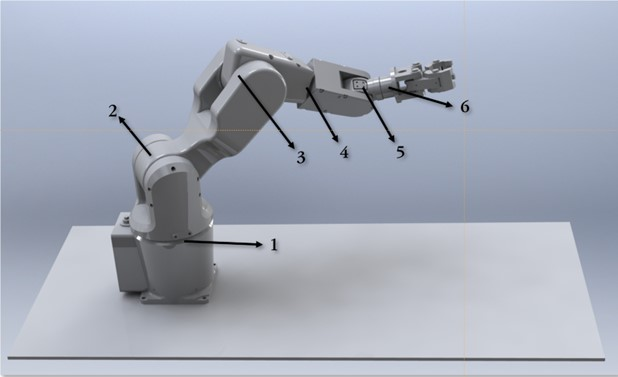
\includegraphics[width=0.8\textwidth]{Image/fig1.jpg}
    \caption{机器人模型和各自由度关节示意图}
    \label{fig:1}    
\end{figure}

我们设计的机器人模型如图\ref{fig:1}所示,可以看到一共7个部分,相互组合一共产生6个自由度,自由度2、3、5为绕水平轴旋转的自由度,自由度1、4、6为绕垂直轴旋转的自由度。最后6个自由度的角度变化驱动最后加持部件的运动,我们的加持部件最后采用了机械夹取手的形式,用来做出灵活的运动,机械夹取手的具体细节如图\ref{fig:2}所示。

\begin{figure}[h]
    \centering
    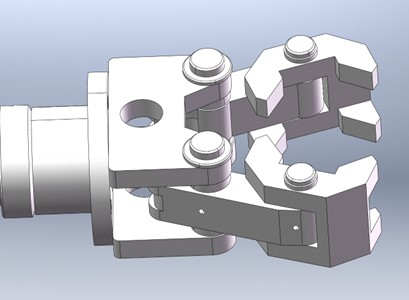
\includegraphics[width=0.8\textwidth]{Image/fig2.jpg}
    \caption{机械夹取手的设计}
    \label{fig:2}
\end{figure}

\subsection{简单运动模拟}
在完成机械臂的建模之后,我们需要模拟机械臂是否已经完成约束配合,能否通过6个自由度上的角度变动带来最后机械臂的自由运动。我们使用了SolidWorks当中的SolidWorks Motion插件,通过这个插件可以让机械臂的末端按照我们规划好的路线运动。我们规划了一个水平圆,让机械臂末端的一个固定点和这个圆进行路径配合,让机械臂的末端绕着这个圆运动。之后利用SolidWorks Motion插件,为这个运动增加了一个路径匹配电机,让机械臂按照制定位置运动。但是也会出现一个问题,机械臂在运动时并没有解决干涉问题。在运动过程中可能存在干涉,导致机械臂出现重合的奇怪现象。目前没有办法能够解决,只能通过调整机械臂的起始姿态和后续的运动距离来避免机械臂重合的现象。

\subsection{运动模拟仿真渲染}
SolidWorks中自带的渲染软件无法完成我们需要的运动渲染,最后我们使用了Keyshot软件。将SolidWorks中已经做好的路径规划导出到Keyshot中,再完成相机布置和运动、背景布置最终完成运动渲染仿真,渲染仿真动画截图如图\ref{fig:3}所示。

\begin{figure}[h]
    \centering
    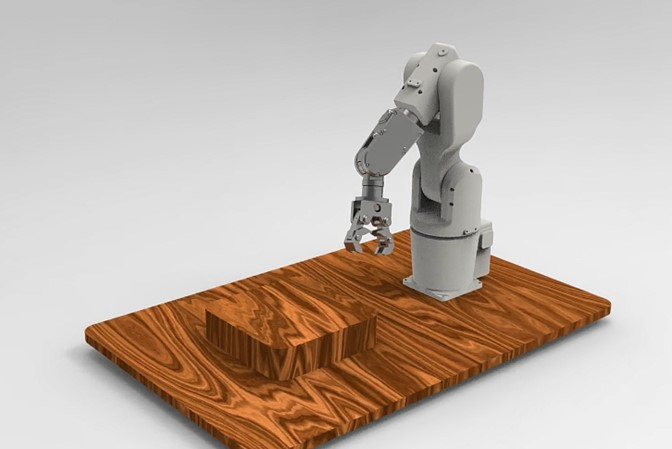
\includegraphics[width=0.8\textwidth]{Image/fig3.jpg}
    \caption{运动仿真渲染}
    \label{fig:3}
\end{figure}

\subsection{应力仿真分析}
最先采用SolidWorks中的Simulation模块进行应力分析,但是在SolidWorks中容易出现网格无法划分的现象,最后使用ANSYS中的静态结构进行应力分析,机械臂的最终采用使用铝合金,因为铝合金具有更轻的重量和比较好的力学表现。在测量机械臂的应力时,我们考虑将机械臂完全伸直,将机械臂在XY平面中伸展到最远,让夹持端受到压力时带来的力矩最大,模拟在最坏的情况下的机械臂应力和形变情况。模拟情况如图\ref{fig:4}所示,红色为受压力较大的地方,颜色越深受到的压力越大,从应力分析的图中可以看到在较细的地方会有更大的应力。

\begin{figure}[h]
    \centering
    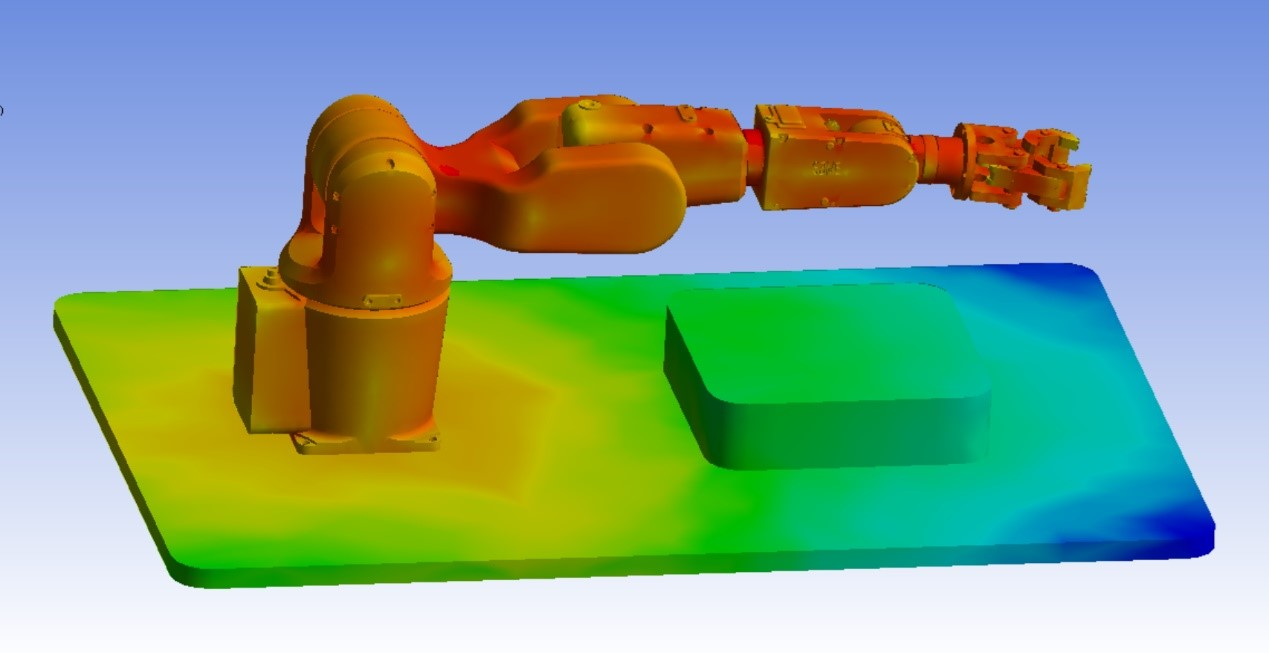
\includegraphics[width=0.7\textwidth]{Image/fig4.jpg}
    \caption{应力分析仿真模拟图}
    \label{fig:4}
\end{figure}

我们还对变形大小进行了分析,模拟情况如图\ref{fig:5}所示,可以看到末端相对于原先位置的位移最大。可以看到最大的变形为0.033472mm,我们可以根据这个数据去计算出位置误差。

\begin{figure}[h]
    \centering
    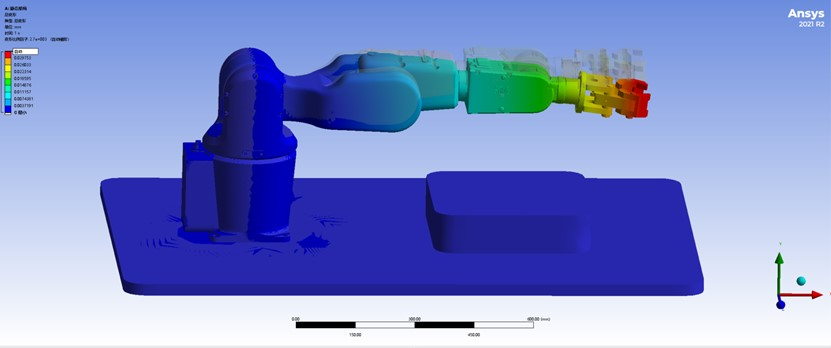
\includegraphics[width=0.7\textwidth]{Image/fig5.jpg}
    \caption{变形分析仿真模拟图}
    \label{fig:5}
\end{figure}

\subsection{误差分析}
在实际应用中,很多因素会影响到机械臂的绝对定位精度,按照定位误差的来源来分类,包括外界环境的变化引起的外部误差和内部结构参数引起的内部误差。

我们调研的结果主要有:
\begin{enumerate}
    \item 结构刚度和变形:
    
    自重:机械臂各个部件的自重会导致结构的弯曲和变形,特别是在机械臂的末端部分,这种效应会更加明显。自重引起的重力作用会使关节和连杆产生变形,导致位置和姿态的误差。

    外力和惯性力:工作过程中受到的外力(如负载和加工力)以及运动时的惯性力也会引起结构变形,导致误差。

    \item 关节误差:
    齿轮传动误差:如果机械臂使用齿轮传动,各个齿轮的制造误差、安装误差和磨损会导致传动精度降低。

    关节间隙:关节中的轴承和传动装置存在间隙,这些间隙在运动过程中会积累误差。

    伺服电机控制精度:电机的控制精度(如分辨率和响应速度)直接影响关节的定位精度。

    \item 传感器误差:
    
    位置传感器精度:用于测量关节角度或位置的传感器(如编码器或电位计)的分辨率和精度会影响定位精度。

    噪声和干扰:传感器信号在传输过程中可能受到电磁干扰和噪声的影响,导致测量数据不准确。
\end{enumerate}

除了以上三种主要的干扰外,误差还来自外界环境的变化包括工作环境中的温度、湿度的变化,电网的冲击,通讯信号的干扰,其他设备的振动,人为因素的干预等;内部由机械臂自身某些部分引起的误差,包括机械臂的运动学参数误差、运动时的摩擦磨损以及润滑条件等。

综合分析以上误差来源,外界环境的变化、受力变形、摩擦磨损等对机械臂的绝对定位精度影响较小,机械臂的运动学参数误差影响较大,由其所导致的误差约占总误差的80\%。

虽然机械臂的定位误差产生原因很多,在理论分析过程中,目前我们能够做到的只有分析机械臂自重所带来的位置误差0.033472mm,这个误差相对于机器人自身的以米为单位的大小这个误差很小,并且我们的重力按照实心重力计算,在使用空心合理优化的情况下机器人自身重量带来的误差会更小。

通过误差传递方程,考虑每一个误差源对于最终结果的敏感性,创建函数:
\begin{equation}
    \varDelta f=\sqrt{\left( \frac{\partial f}{\partial x_1}\Delta x_1 \right) ^2+\left( \frac{\partial f}{\partial x_2}\Delta x_2 \right) ^2+\cdots +\left( \frac{\partial f}{\partial x_n}\Delta x_n \right) ^2}
\end{equation}

这里,$\frac{\partial f}{\partial x_i}$是$f$对$x_i$的偏导数, $\Delta x_i$是$x_i$的误差。从公式中可以看到随着产生误差变量的增多,系统的误差会逐渐增大,并且相对于不同的误差,会有不同的计算权重来进行叠加。以简单的双关节机械臂来看,假设其两个关节角分别为$\theta_1,\theta_2$连杆长度分别为$l_1,l_2$,由末端位置可以得到正向运动学方程,

\begin{equation}
    \left\{ \begin{array}{c}	x=l_1cos\left( \theta _1 \right) +l_2cos\left( \theta _1+\theta _2 \right)\\	y=l_1sin\left( \theta _1 \right) +l_2sin\left( \theta _1+\theta _2 \right)\\\end{array} \right. 
\end{equation}

假设角度和长度都存在误差$\Delta\theta_1,\Delta\theta_2,\Delta l_1,\Delta l_2$,则根据误差传递函数可以得到统计结果:

\begin{equation}
    \begin{aligned}
    \varDelta x &=\sqrt{\left( \frac{\partial x}{\partial \theta _1}\Delta \theta _1 \right) ^2+\left( \frac{\partial x}{\partial \theta _2}\Delta \theta _2 \right) ^2+\left( \frac{\partial x}{\partial l_1}\Delta l_1 \right) ^2+\left( \frac{\partial x}{\partial l_2}\Delta l_2 \right) ^2}\\
    \varDelta y &=\sqrt{\left( \frac{\partial y}{\partial \theta _1}\Delta \theta _1 \right) ^2+\left( \frac{\partial y}{\partial \theta _2}\Delta \theta _2 \right) ^2+\left( \frac{\partial y}{\partial l_1}\Delta l_1 \right) ^2+\left( \frac{\partial y}{\partial l_2}\Delta l_2 \right) ^2}
    \end{aligned}
\end{equation}

通过这些计算就可以得到最终的误差,通过识别不同的误差源并且建立适当的误差传递方程就可以得到能正确反映机器人误差的方程。对于我们的六自由度协作机器人,我们的单一误差就能达到12个,再加上不同关节角度和连杆长度所产生的误差也是由其他的误差叠加产生,就会产生一个非常复杂的误差传递方程。

想要减少误差我们可以采用一下几种办法:

\begin{itemize}
    \item 采用高刚度材料和结构设计,减少变形,针对由于自重变形部分的误差进行误差减小。
    \item 提高传动装置和传感器的制造和装配精度,通过对装配误差的控制,减小不可控的精度差。
    \item 使用补偿算法,校正因温度变化和其他因素引起的误差,通过误差补偿,直接针对系统的误差进行校正。
    \item 优化控制算法,提高控制系统的响应速度和稳定性,同时可以减小运动过程中对于机械臂的磨损,让精度长时间保存。
    \item 定期维护和校准机械臂,确保其各部分处于最佳状态,对其中影响误差的部分进行修复确保精度正确。
\end{itemize}

以上方法可以通过控制误差方程中的一个或者多个误差来减小整体的误差,对于误差的调整程度需要对于实际的机器人进行具体的分析。

\section{材料与选型}
\subsection{材料选择}
材料选择方面,我们收集了市面上常见机器人材料的资料,其优缺点对比情况如\ref{fig:6}所示。在各连杆材料选择时,我们需要综合考虑材料密度、刚度、强度、成本等多方面因素。

\begin{figure}[h]
    \centering
    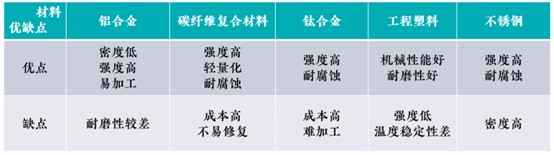
\includegraphics[width=0.7\textwidth]{Image/fig6.jpg}
    \caption{常见机器人材料优缺点对比}
    \label{fig:6}
\end{figure}

最终我们选取了不锈钢作为底座,其具有足够的强度和密度,足以稳定机身;选取了中空的铝合金作为机器人杆件、关节的材料,该材料能兼顾强度、刚度、重量,且中空的结构使机器人从法兰到底座能够全程内部走线。

\subsection{电机、减速器选型}
考虑到机器人关节速度不能过大,统一电机的额定转速为3000 r/min,故初步选取减速比i=100的谐波减速机。	

在机器人末端施加6kg负载,通过动力学的计算,可得出机器人需要的额定转矩估值,以此为依据为机器人各关节选取合适的电机和减速机。

选取结果如表\ref{tab:1}所示:

\begin{table}[h]
    \centering
    \caption{电机、减速器选型}
    \label{tab:1}
    \vspace{5pt}
    \begin{tabular}{cccccc}
    \rowcolor[HTML]{4472C4} 
    关节 & \begin{tabular}[c]{@{}c@{}}额定转矩\\ (Nm)\end{tabular} & \begin{tabular}[c]{@{}c@{}}减速机型号\\ (i=100)\end{tabular} & \begin{tabular}[c]{@{}c@{}}额定转矩\\ (Nm)\end{tabular} & 电机型号             & \begin{tabular}[c]{@{}c@{}}电机额定功率\\ (Nm)\end{tabular} \\
    \rowcolor[HTML]{D9E2F3} 
    1  & 60                                                  & SHXB-CSF-25-A                                           & 0.6                                                 & SM 60-006-30 LFB & 0.2                                                   \\
    2  & 67                                                  & SHXB-CSF-25-A                                           & 0.67                                                & SM 60-006-30 LFB & 0.2                                                   \\
    \rowcolor[HTML]{D9E2F3} 
    3  & 30                                                  & SHXB-CSF-20-A                                           & 0.3                                                 & SM 40-003-30 LFB & 0.1                                                   \\
    4  & 65                                                  & SHXB-CSF-25-A                                           & 0.65                                                & SM 60-013-30 LFB & 0.4                                                   \\
    \rowcolor[HTML]{D9E2F3} 
    5  & 100                                                 & SHXB-CSF-32-A                                           & 1                                                   & SM 80-013-30 LFB & 0.4                                                   \\
    6  & 60                                                  & SHXB-CSF-25-A                                           & 0.6                                                 & SM 60-006-30 LFB & 0.2                                                  
    \end{tabular}
    \end{table}
    
    图\ref{fig:7}展示了我们选用的主要型号的减速器的工程图,图\ref{fig:8}展示了我们选用的主要型号的电机实物图。
\begin{figure}[h]
    \centering
    \subfigure[减速器工程图]{
    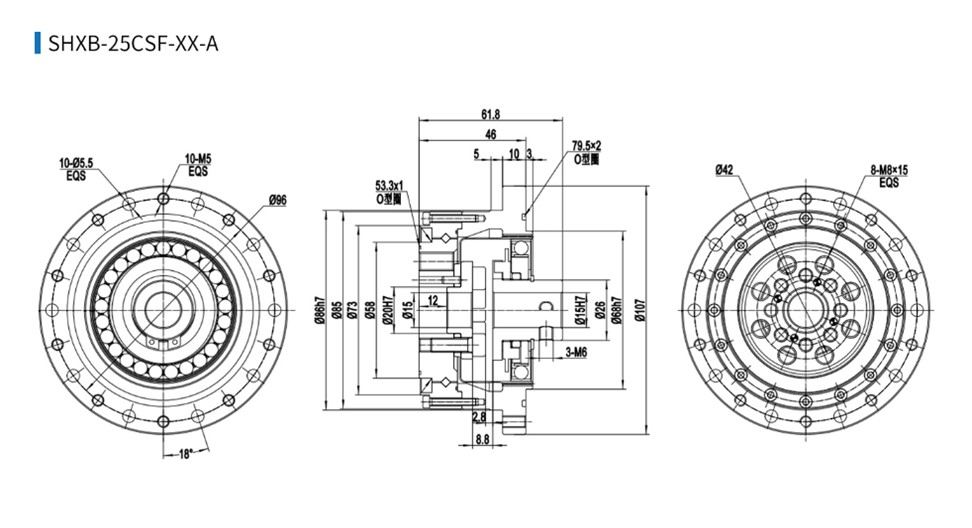
\includegraphics[width=0.5\textwidth]{Image/fig7.jpg}
    \label{fig:7}
    }
    \subfigure[电机实物图]{
    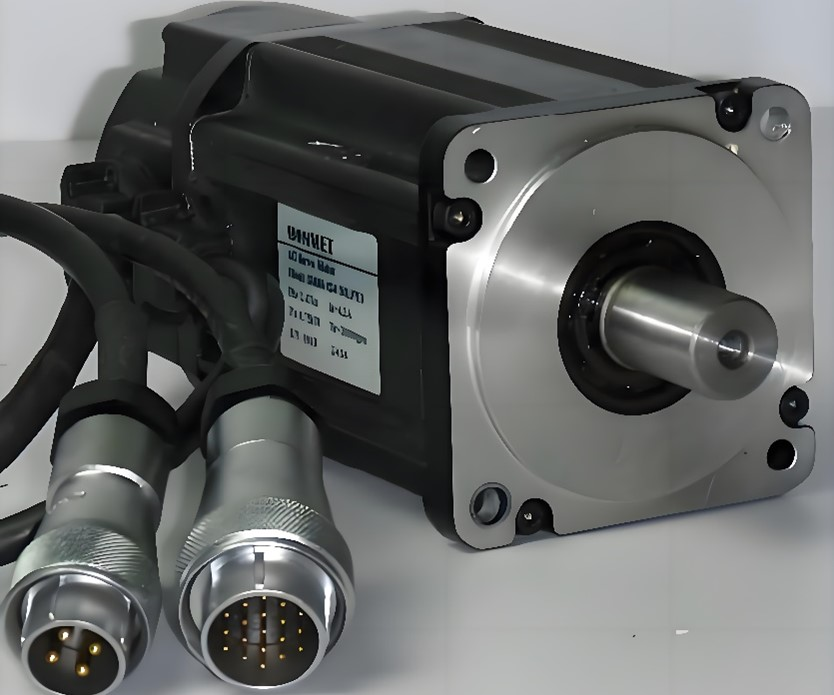
\includegraphics[width=0.4\textwidth]{Image/fig8.jpg}
    \label{fig:8}
    }
    \caption{减速器和电机选型}
\end{figure}
\newpage

\section{工作空间}
\subsection{背景介绍}
机器人的工作空间是评价机器人工作性能的一项重要指标。工作空间分为可达工作空间和灵巧工作空间。可达工作空间是指机器人末端执行器参考点所能到达的位置的集合。

机器人工作空间是机器人设计与优化的重要依据。王晓华等以六轴缝纫机器人为对象,通过对机器人末端的可达工作空间分析确定了缝纫机器人在工作时各关节的最佳运动范围。荆学东等以六轴双臂服务机器人为对象,求解了双臂各自的可达工作空间,以协作空间最大为优化目标,对机器人的结构参数进行了优化。赵智远等研制了 9 自由度超冗余串联机械臂,以可达工作空间与灵活工作空间为优化目标,对机械臂的构型进行了优化设计。贾世元等以六轴机械臂为对象,以全局灵活性为优化目标,对机械臂尺寸参数进行了优化设计。

目前,求解机器人工作空间的方法主要有3类:几何法、解析法和数值法:
\begin{itemize}
    \item \textbf{几何法}可以得到机器人的解剖面或解剖线,但受到自由度数的限制,无法精确描述多自由度机器人的工作空间,主要用于平面机器人的求解。
    \item \textbf{解析法}是通过多次包络求解机器人工作空间的方法,可以求出工作空间边界的数学方程,但求解过程复杂,主要用于关节数量少于3个的机器人。
    \item \textbf{数值法}是将多个关节角组合代入到正向动力学方程,求解出机器人末端在任务空间的坐标,最终得到工作空间的方法,求解简单,适用于任意结构的机器人工作空间的求解。
\end{itemize}

在数值方法中,求解机器人工作空间最为常见的方法就是蒙特卡洛方法。传统蒙特卡洛法的主要问题是工作空间点分布不均匀,大部分工作空间点产生在工作空间内部,导致工作空间边界求取精度不高,当提高工作空间点数量以提升工作空间边界求取精度时,大量工作空间点任然出现在工作空间内部,造成了计算资源的浪费,导致求解速度较慢。针对上述问题,徐振邦等利用蒙特卡洛法生成了一个种子工作空间,对于每个工作空间点数量较少的位置,在其内部选取一个参考点,在生成该点的关节角附近多次随机抽样并代入正向运动学方程,一次性得到多个工作空间点。这种方法使工作空间点云密度分布更加均匀,提高了工作空间边处的精确度,但该方法的求解效率与分块数有关,需要根据具体的结构进行调整,并且拓展得到的工作空间点过于集中。刘志忠等先利用蒙特卡洛法生成了一个种子空间,对种子空间分层,寻找每层的边界点,在边界点附近生成多个随机点,多次迭代,直到形成精确的边界。这种方法提高了工作空间边界处的精度,但求解精度依赖于分层数量,分层过少时精度不高,分层过多时消耗时间长。

在本项目中,我们参考李星辰提出的改进的蒙特卡洛方法,利用传统蒙特卡洛法生成种子空间,拓展随机点数量较少的子空间,动态调整正态分布概率密度函数的参数,得到了可达工作空间。

\subsection{传统Mento Carlo方法}
蒙特卡洛法是一种基于概率统计理论,用于模拟随机现象的数值方法。在求解机器人工作空间时,在各个关节角取值范围内随机抽取大量的关节角变量值进行组合,将这些关节角值组合带入正向运动学方程,计算出机器人末端执行器参考点的坐标值,这些参考点所包络的空间就是机器人工作空间。

传统蒙特卡洛法存在的问题如下:求解机器人工作空间时,工作空间边界的具体位置由工作空间边界的参考点给出,工作空间内部的点意义不大。然而,虽然传统蒙特卡洛法随机抽取的关节角值服从均匀分布,但关节空间到工作空间的映射是非线性的,大量工作空间点出现在工作空间内部,导致工作空间的精度不高。当增加随机抽取的关节角值组合的数量时,大部分参考点任然出现在非工作空间边界部分,虽然工作空间的精度变高,但大量的工作空间点没有意义,造成了计算资源的浪费。

\subsection{改进Mento Carlo方法}
针对上述问题,我们再项目中提出一种改进的蒙特卡洛法,该方法由3个部分组成:
\begin{enumerate}
    \item 生成种子空间。利用传统蒙特卡洛法生成大量的工作空间点,用长方体包络所用种子空间点,划分成数个相等的子空间。
    \item 拓展种子空间。筛选出需要拓展的子空间,利用正态分布抽样对这些子空间拓展,同时设置一个精度阈值确保拓展后的工作空间足够准确。为了保证拓展产生的点出现在边界附近,正态分布概率密度函数的方差会根据拓展后的点的位置进行调整。 
    \item 输出可达工作空间。多次重复拓展过程,直到每个子空间得到精确描述,输出可达工作空间。
\end{enumerate}

工作流程图可参考图\ref{fig:9}。

\begin{figure}[h]
    \centering
    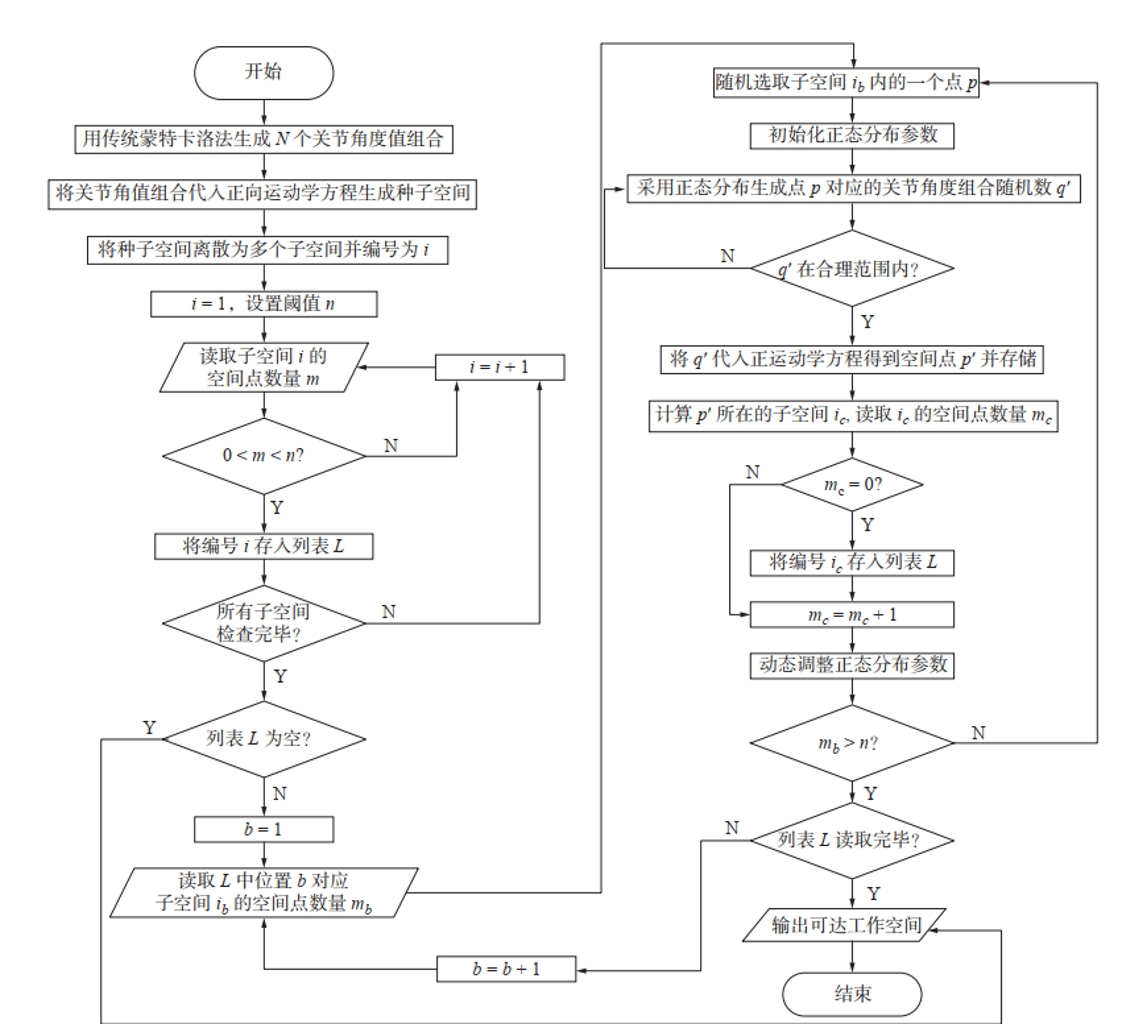
\includegraphics[width=0.8\textwidth]{Image/fig9.jpg}
    \caption{改进Menlo Carlo方法工作流程图}
    \label{fig:9}
\end{figure}

具体的详细步骤如下:
\newpage
\begin{enumerate}
    \item \textbf{生成种子空间} 
    
    用传统蒙特卡洛法对每一关节生成N个随机角度值,按序号组成对应关节角值组合。将关节角值组合代入正向运动学方程,求解出工作空间点在三维笛卡尔坐标系中的坐标值 ,记录参考点在3个坐标轴方向的最大值和最小值,并分别表示为$X_{max},X_{min},Y_{max},Y_{min},Z_{max},Z_{min}$。
    
    将求得的长方体分别沿 3 个坐标轴方向分成$n_x,n_y,n_z$等距部分,整个长方体被分成了$k=n_x\times n_y\times n_z$ 个相等的子空间,根据每个子空间的位置进行编号,存储每个子空间内的工作空间点数量$m$,并存储每个工作空间点的位置信息以及关节角信息。
    \item \textbf{拓展种子空间}
    
    为了在提高可达工作空间边界求取精度时,减少计算资源的浪费,并且方便灵活工作空间的求解,应对每个工作空间点数量较少的子空间进行拓展。设置工作空间点数量阈值$n$,对每个子空间判断,若子空间内包含工作空间点并且工作空间点数量$<n$,则该子空间需要拓展,将该子空间的编号存入列表$L$;否则,不存入列表。所有子空间检查完毕后,对列表$L$进行判断,若列表$L$不为空,则对所有与列表$L$中编号对应的子空间进行拓展;否则,输出可达工作空间。
    
    对每一个需要拓展的子空间$i$,随机抽取一个该子空间内部的工作空间点p,找到与该点对应的关节角值组合q。在关节角值组合$q$附近利用正态分布概率密度函数选取随机值,均值$\mu=q$,标准差初始值依据具体情况进行设定。取值后对新空间点的合理性进行判断,若关节角值组合q的每个关节角值都在该关节角的取值范围内,则保留该取值;若不满足,则舍弃该次取值并重新取值。将取得的关节角值组合$q\prime$代入正向运动学方程,产生一个新的工作空间点$p\prime$,并存储新生成工作空间点的位置信息和关节角信息。为了使得每个本应存在工作空间点的子空间均得到拓展,计算出工作空间点$p\prime$所在的子空间$i_c$,读取子空间$i_c$的工作空间点数量$m_c$,对其进行判断,若$m_c=0$,则将子空间存入列表$L$。为了避免拓展后的工作空间点集中出现在一个工作空间点附近,每拓展一次后进行判断,若该子空间中的工作空间点数量小于阈值$n$,则重新在该子空间中的工作空间点中任意抽取一个点$p$,重复拓展过程,直到该子空间中的工作空间数量大于阈值$n$。

    由于部分子空间与实际工作空间的交集较小,在拓展这一类子空间时,新生成的点$p\prime$虽然大部分出现在被拓展点$p$附近,却出现在被拓展点$p$所在的子空间之外,导致该子空间附近的子空间产生大量的工作空间点,造成了计算资源的浪费。同时,部分位于关节角范围边界处的关节角值组合q,在产生新的关节角值组合$q\prime$时,$q\prime$常常出现在关节角取值范围外,需要重新取值,造成了资源的浪费。为了减少上述的计算资源的浪费,需要根据新生成的关节角值$q\prime$和工作空间点$p\prime$的位置调整正态分布的方差$\sigma$。用$n_f$代表拓展时新生成的关节角值在对应关节角取值范围外的次数,用$n_l$代表拓展时新生成的工作空间点出现在被拓展点p所在子空间外的次数,当$n_f$大于临界值$n_f^{max}$时,表明正态分布方差$\sigma$过大,将正态分布方差$\sigma$除以一个大于1的数$\delta$以缩小方差$\sigma$,方差$\sigma$调整后,将$n_f$置零;当$n_l$大于临界值$n_l^{max}$时,表明该子空间与实际工作空间的交集较小,将正态分布方差$\sigma$除以一个大于1的数$\delta$以缩小方差$\sigma$,方差$\sigma$调整后,将$n_l$置零。每拓展完一个子空间后,$n_f,n_l$置零。
    \item \textbf{输出可达工作空间}
    
    列表L中的子空间全部拓展后,每个子空间已得到精确描述,得到可达工作空间,输出存储的点的位置信息。
\end{enumerate}

\subsection{实例求解}
基于我们小组的机械臂模型参数,我们分别用传统蒙特卡洛法和本文所述的改进蒙特卡洛法在 MATLAB 编程,进行工作空间求解仿真,并利用 MATLAB 中的拟合函数求解工作空间体积。

首先设置改进的蒙特卡洛法参数,如表\ref{tab:2}所示:

\begin{table}[h]
    \centering
    \caption{改进蒙特卡洛法参数设置}
    \vspace{5pt}
    \label{tab:2}
    \begin{tabular}{
    >{\columncolor[HTML]{ECF4FF}}c 
    >{\columncolor[HTML]{ECF4FF}}c 
    >{\columncolor[HTML]{ECF4FF}}c 
    >{\columncolor[HTML]{ECF4FF}}c 
    >{\columncolor[HTML]{ECF4FF}}c 
    >{\columncolor[HTML]{ECF4FF}}c 
    >{\columncolor[HTML]{ECF4FF}}c }
    \hline \hline
    N     & k        & n  & $\sigma$ & $\delta$ & $n_f^{max}$ & $n_l^{max}$ \\ \hline
    10000 & 20*20*20 & 50 & $\pi/3$  & 1.5      & 5           & 300         \\ \hline\hline
    \end{tabular}
    \end{table}

其中,N是初始生成的种子数,k是划分的子空间的数量,n是设置的工作子空间点数量阈值,$\sigma$是方差,$\delta$是一个大于1的参数,$n_f^{max}$新生成的关节角值在对应关节角取值范围外的次数的最大值,$n_l^{max}$新生成的工作空间点出现在被拓展点p所在子空间外的次数的最大值。

\textbf{下面进行相同工作空间点数下的比较}:下面四张图片分别展示了传统的蒙特卡洛方法与改进的蒙特卡洛方法求解的工作空间的示意图,可以清楚的看到,在生成的工作点数均为$1000000$左右的情况下,传统的蒙特卡洛方法生成的工作空间的边界粗糙、模糊、像是像素低一般,而改进的蒙特卡洛方法生成的工作空间的边界圆润、清晰,效果较好。

\begin{figure}[h]
    \centering
    \subfigure[传统蒙特卡洛法工作空间示意图1]{
    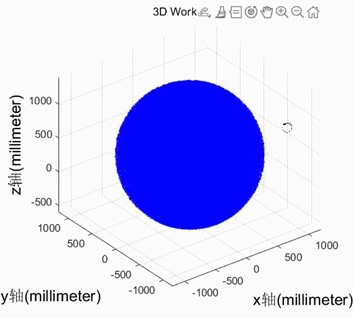
\includegraphics[width=0.4\textwidth]{Image/fig10.jpg}
    }
    \subfigure[传统蒙特卡洛法工作空间示意图2]{
    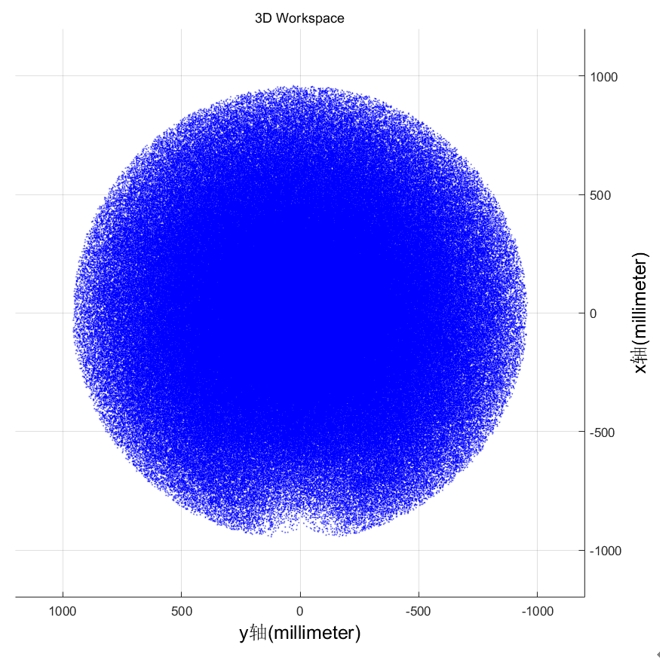
\includegraphics[width=0.4\textwidth]{Image/fig11.png}
    }
    \caption{传统蒙特卡洛法工作空间示意图}
    \label{fig:10}
\end{figure}


\begin{figure}[h]
    \centering
    \subfigure[改进蒙特卡洛法工作空间示意图1]{
    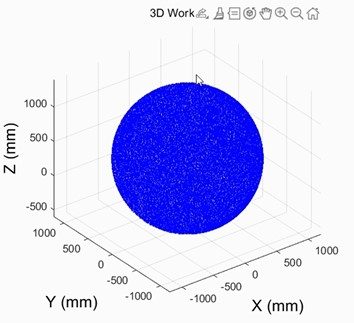
\includegraphics[width=0.4\textwidth]{Image/fig12.jpg}
    }
    \subfigure[改进蒙特卡洛法工作空间示意图2]{
    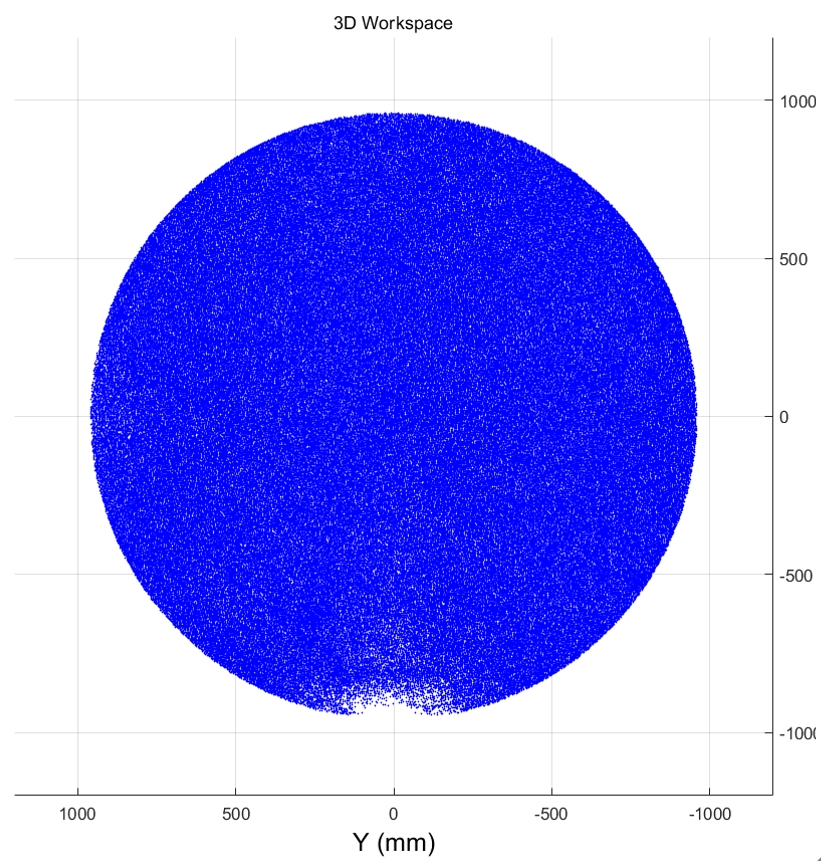
\includegraphics[width=0.4\textwidth]{Image/fig13.jpg}
    }
    \caption{改进蒙特卡洛法工作空间示意图}
    \label{fig:11}
\end{figure}

\textbf{对不同空间工作点数下传统的蒙特卡洛方法进行比较}:

通过不断增加传统蒙特卡洛法的随机工作空间点数量,使求解得到的工作空间越来越接近实际工作空间。用生成的工作空间体积变化表示工作空间的变化,逐渐增加工作空间点数量,工作空间的体积随工作空间点数量增加的变化如表\ref{tab:3}所示:

\begin{table}[h]
    \centering
    \caption{传统方法求得的可达工作空间体积随工作空间点数数量的变化}
    \vspace{5pt}
    \label{tab:3}
    \begin{tabular}{
    >{\columncolor[HTML]{FFFFC7}}c |
    >{\columncolor[HTML]{FFFFC7}}c |
    >{\columncolor[HTML]{FFFFC7}}c |
    >{\columncolor[HTML]{FFFFC7}}c |
    >{\columncolor[HTML]{FFFFC7}}c |
    >{\columncolor[HTML]{FFFFC7}}c |
    >{\columncolor[HTML]{FFFFC7}}c |
    >{\columncolor[HTML]{FFFFC7}}c }
    \hline \hline
    N       & $5000$ & $10^4$ & $5\times 10^4$ & $10^5$ & $5\times 10^5$ & $10^6$ & $10^7$ \\ \hline
    $V/m^3$ & 3.3486 & 3.4374 & 3.5791         & 3.6104 & 3.6615         & 3.6740 & 3.6950 \\ \hline \hline
\end{tabular}
\end{table}

从表\ref{tab:3}可以看出,当工作空间点数达到1000000时,体积不再明显变化,体积为3.6950 $m^3$;采用改进方法求解,当体积达到3.6947$m^3$时,仅需要422458个工作点,所以需要的点数仅为传统方法的4.22\%,求解效率大大提高。

传统的蒙特卡洛方法生成的工作空间的边界如图\ref{fig:10}所示,改进的蒙特卡洛方法生成的工作空间的边界如图\ref{fig:11}所示,可以看出改进的蒙特卡洛方法生成的工作空间的边界更加清晰、圆润,效果更好。

对于不同点数的工作空间的示意图如图\ref{fig:12}所示,可以看出,随着工作空间点数的增加,工作空间的边界越来越清晰,更加接近实际工作空间,出于实际排版美观的考虑,将图片放在下页。

\begin{figure}[htbp]
    \centering
    \subfigure[$N=5000$]{
    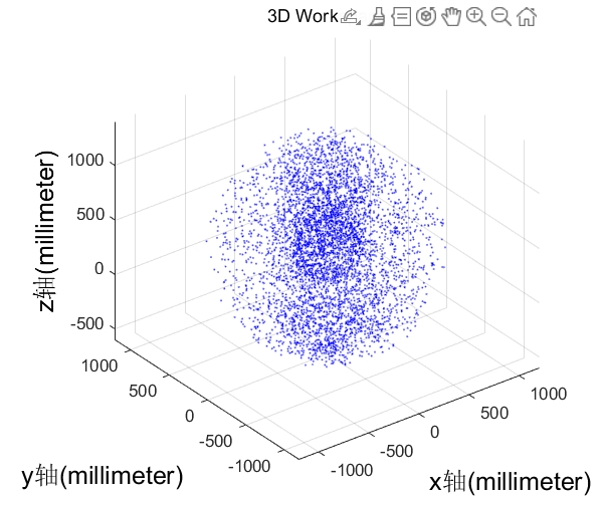
\includegraphics[width=6cm]{Image/fig14.jpg}
    }
    \quad
    \subfigure[$N=10^4$]{
    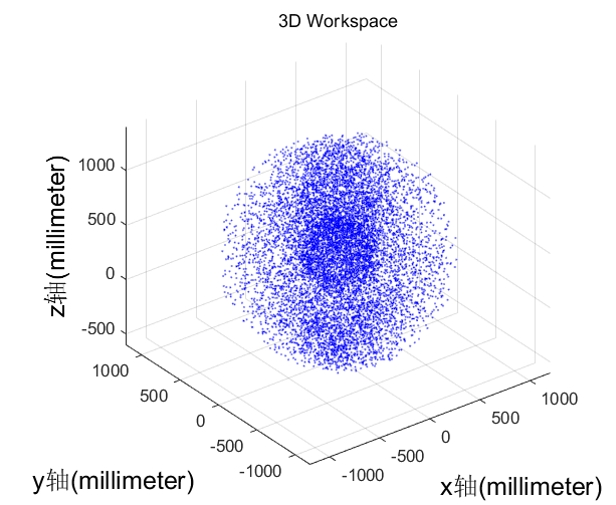
\includegraphics[width=6cm]{Image/fig15.jpg}
    }
    \quad
    \subfigure[$N=5\times 10^4$]{
    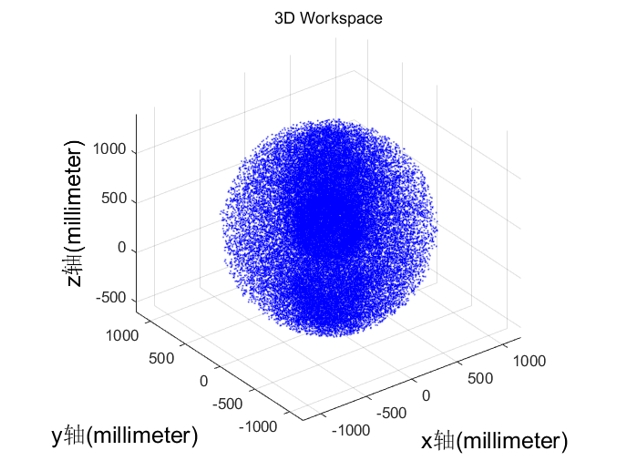
\includegraphics[width=6cm]{Image/fig16.jpg}
    }
    %\caption{fig1}
    \quad
    \subfigure[$N=10^5$]{
    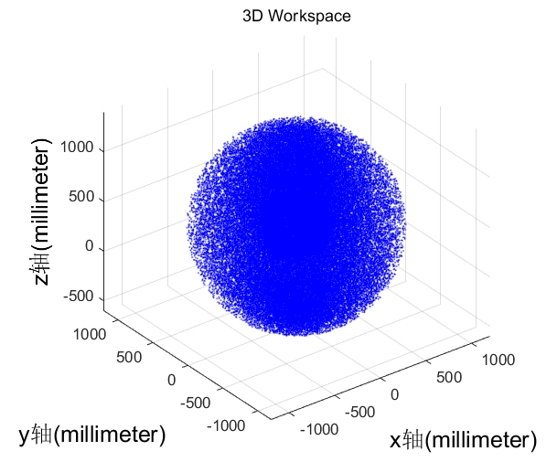
\includegraphics[width=6cm]{Image/fig17.jpg}
    }
    \quad
    \subfigure[$N=5\times 10^5$]{
    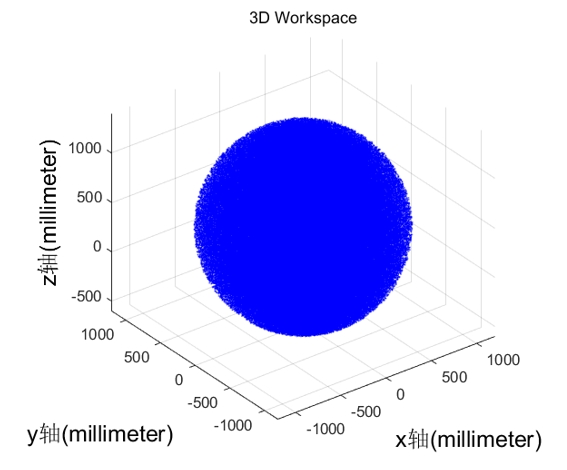
\includegraphics[width=6cm]{Image/fig18.jpg}
    }
    \quad
    \subfigure[$N=10^6$]{
    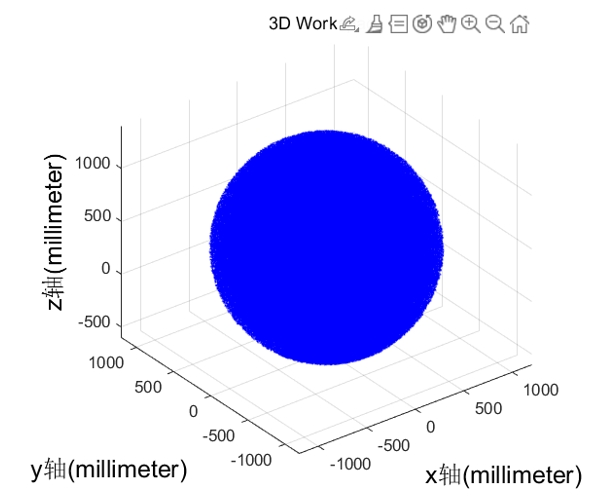
\includegraphics[width=6cm]{Image/fig19.jpg}
    }
    \caption{不同N下工作空间的示意图}
    \label{fig:12}
    \end{figure}
